\documentclass[print,onecolumn]{revtex4-1}
\usepackage{hyperref}
\usepackage{graphicx}
\usepackage{url}
\graphicspath{{images/}}


\begin{document}

\title{Computational Physics (Physics.566.01.Sp15)--Group Assignment}
\author{Tong Zhu (NetID: tz37)}
\affiliation{Mechanical Engineering \& Materials Science, Duke University}
\email[E-mail me:]{tz37@duke.edu}
\date{\today}
\maketitle

\section{Introduction}
In this part, we will do some research about the correlation between the fraction F and the occupation probability p. Former studies show that the correlation between the occupation probability p and the fraction is under a power-law ansatz: 
\begin{eqnarray}
F(p>p_c)& = & \frac{no.\  of\  sites \ in\  spanning\  cluster}{no. \ of \ occupied \ sites} \nonumber \\
F&=&F_0(p-p_c)^\beta
\end{eqnarray}


\section{Method}


For the implementation, my code flow is like below:
\begin{itemize}
\item Set a grid list, and a list that can be chosen (Vacancy list). 
\item Randomly choose a Vacancy, and put an particle in that Vacancy according to the occupation probability. 
\item if the position have a particle, combine two junk clusters after that set.
\item  Repeat former steps, until whole grid have been chosen once. 
\end{itemize}

In this way, we use a tuple in python to keep all the cluster list, and their x coordinate and y coordinate. 


\section{Results}

According to the former study (Problem a)), we have know that the critic occupation probability for 100 lattice size is near 0.59, by set p from 0.60 to 0.90 (30 points total), we get correlation between  fraction and occupation probability shown in Fig. \ref{tong1}

\begin{figure}[htbp]
\begin{center}
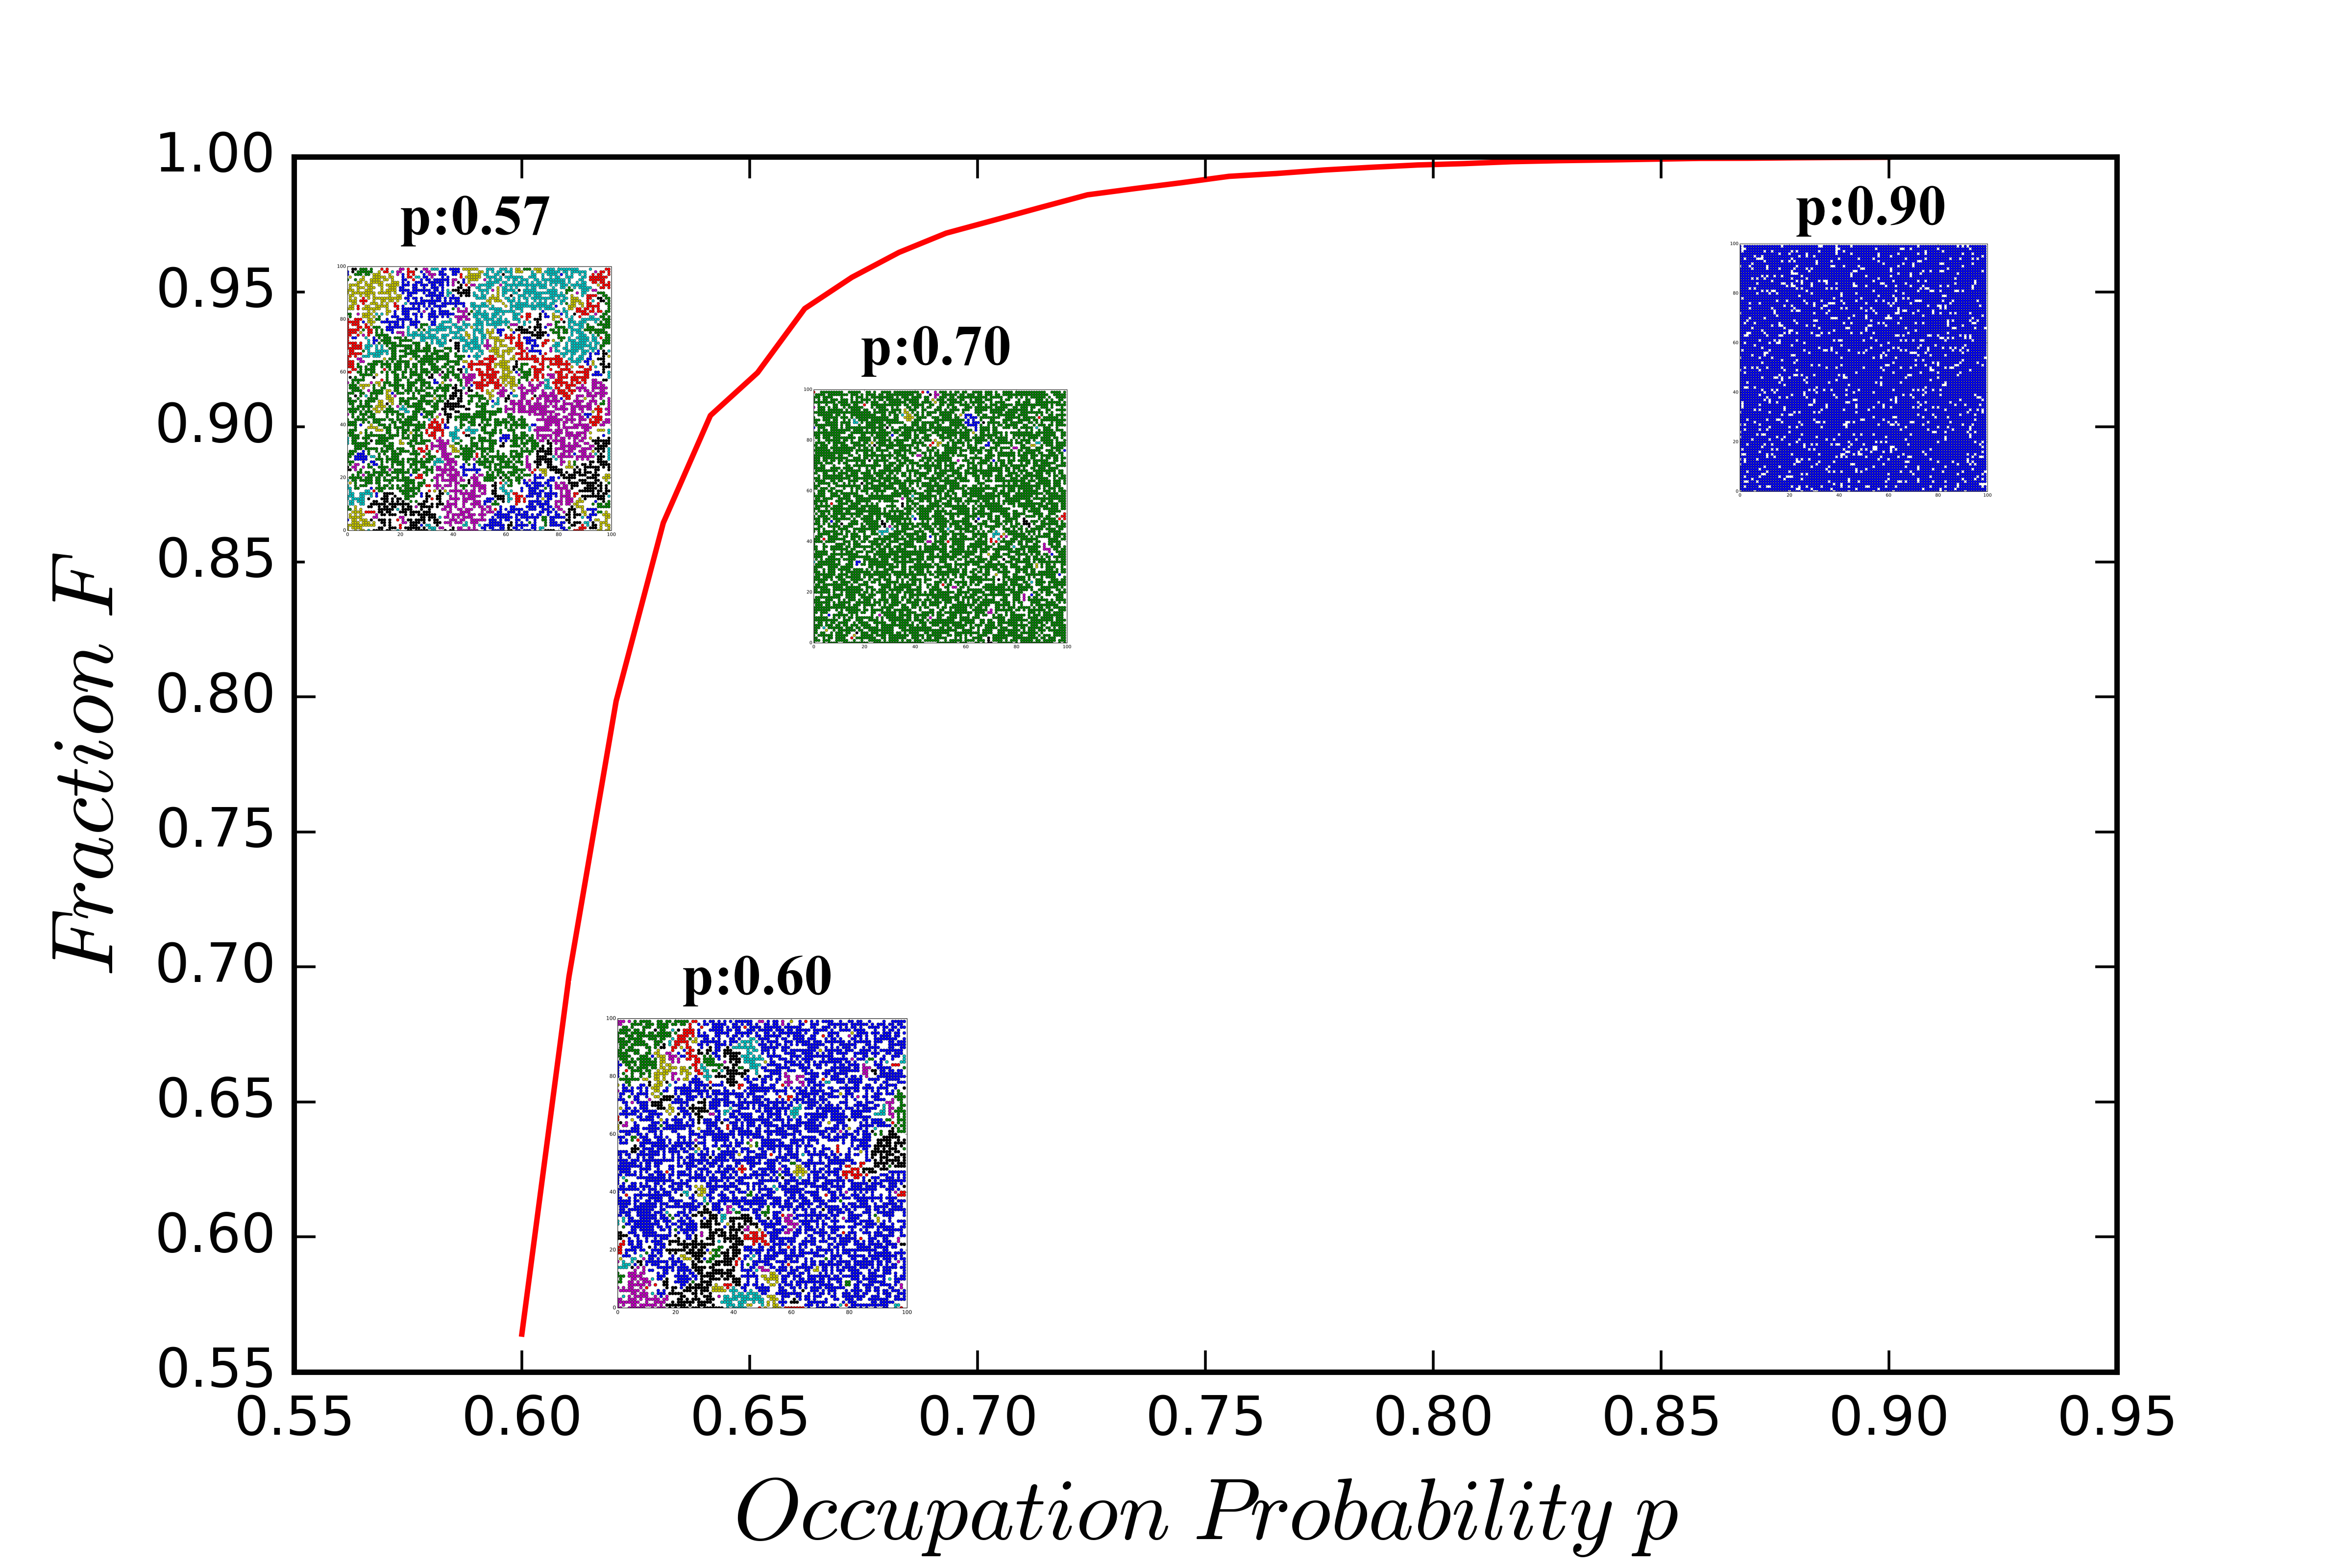
\includegraphics[width=14cm]{P1.png}
\caption{The correlation between occupation probability p and fraction F, the cluster forms under different occupation probability are shown in this figure.}
\label{tong1}
\end{center}
\end{figure}



From this figure, we find that as the occupation growing, the fraction number would quckily goes to its limit 1, and we can see this by the formation of clusters clearly. When  p below the critical occupation number p$_c$,  it shows different kinds of clusters (p:0.57), but when it higher than p$_c$, the span cluster becomes major, and it seems it always have just one span clusters. When the occupation number becomes too high, there is only one span cluster which occupy the whole area (p:0.90). 

By seeing the cluster formation near the critical occupation probability shown in Fig. \ref{tong2}, we know that in this case, it will have no span cluster cases(left side).

\begin{figure}[htbp]
\begin{center}
\includegraphics[width=14cm]{cluster.png}
\caption{The cluster forms at occupation probability 0.59. The left one are showing no span cluster case, the right one are showing span cluster case.}
\label{tong3}
\end{center}
\end{figure}



By choosing the range from 0.60 to 0.65, we do a fit according to the power ansatz function shown in Fig. \ref{tong3}

\begin{figure}[htbp]
\begin{center}
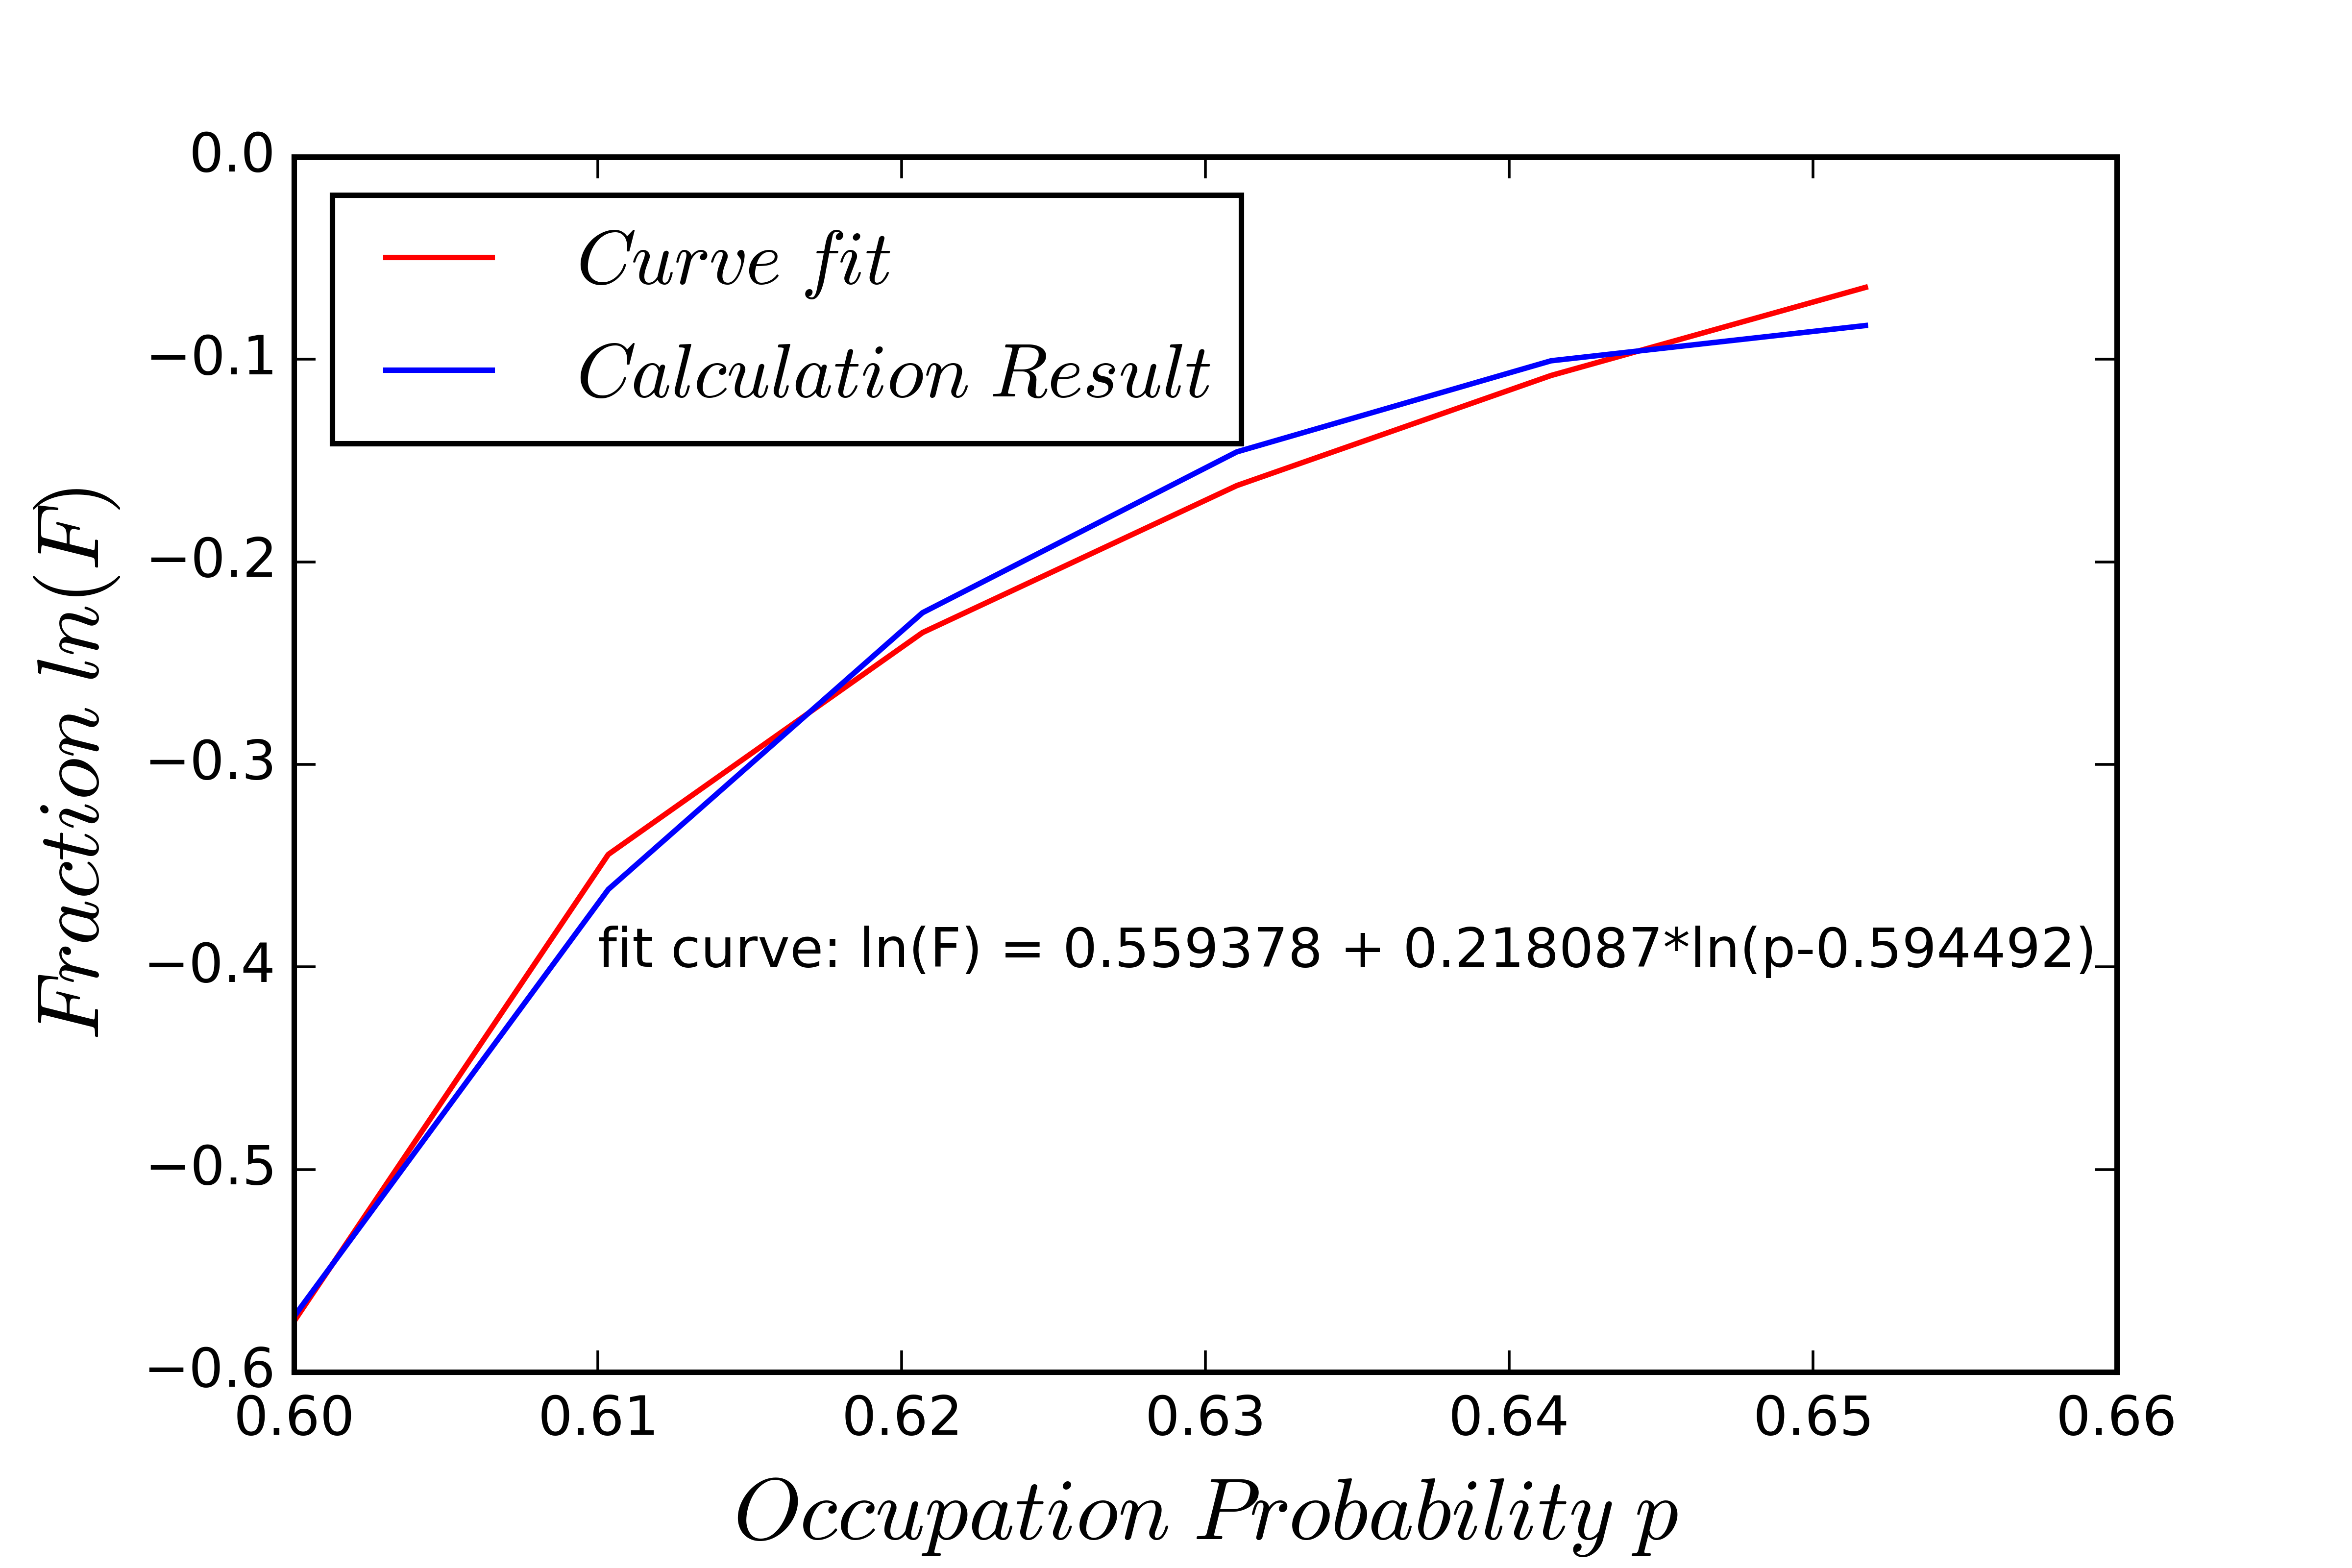
\includegraphics[width=14cm]{P2.png}
\caption{The analysis doing from occupation probability 0.6 to 0.65.}
\label{tong3}
\end{center}
\end{figure}


From our fit parameter, we can see that the $\beta$ = 0.218087, and the p$_c$=0.594492, F$_0$=e$^0.559378$=1.749583


\end{document}